\documentclass{article}
\usepackage[utf8]{inputenc}
\usepackage{graphicx}

\title{Computational Physics (physics760) \\ Exercise 1}
\author{Ajay S. Sakthivasan, Dongjin Suh}
\date{October 28, 2022}

\begin{document}

\maketitle

\section{Simulation of the 1D Ising Model}
\begin{enumerate}
    \item $J$ is the interaction coefficient, and determines the strength of interaction between two adjacent lattice points. It's apparent from the Hamiltonian that $J = 0$ corresponds to a system in which there's no interaction between different points in the lattice. In such cases, the Hamiltonian has only one possible non-zero contribution, which is from the energy due to the external field. Further, $J>0$ corresponds to ferromagnets, where the spins desire to be aligned (neighbouring spins have same signs). And, $J<0$ corresponds to antiferromagnets, where the spins desire to anti-aligned (neighbouring spins have opposite signs).
    \item There are two different types of boundary conditions that can be imposed on the system, \textit{free} and \textit{periodic}. In free boundary condition, the spins at the boundary of the system interact only with the nearest interior spins. Whereas, in the periodic boundary condition, they also interact with the spins topologically next to them, as if the system had a modulo N labelling for the spins. For example, in the 1D Ising model, we get terms like $-J\sigma_1\sigma_N$ in the Hamiltonian, which is absent in the free boundary condition.
    \item Since we are working in the unites with $k_B = 1$, the relevant dimensionless quantity is $\frac{\mathcal{H}(s)}{T}$, or equivalently, any term of the form $\frac{[Energy]}{[Temperature]}$, i.e., $[Energy]$ and $[Temperature]$ have the same dimension.\\
\begin{figure}[h!]
    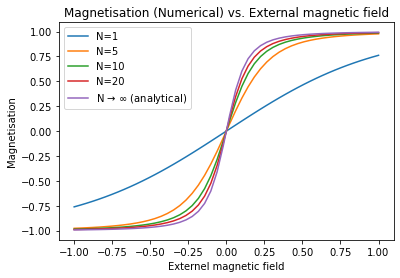
\includegraphics[width=.45\textwidth]{mh-numerical.png}\hfill
    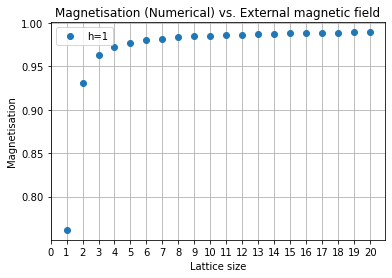
\includegraphics[width=.45\textwidth]{mn-numerical.png}\hfill
    \caption{Magnetisation calculated using brute-force method}
    \label{fig:numerical}
\end{figure}
    In figure \ref{fig:numerical}, we have the plots obtained for magnetisation using brute-force method. The first subplot shows the magnetisation for different values of the external field. Whereas, the second subplot shows the magnetisation for different lattice sizes with the external magnetic field set at $1$.\\
\begin{figure}[h!]
    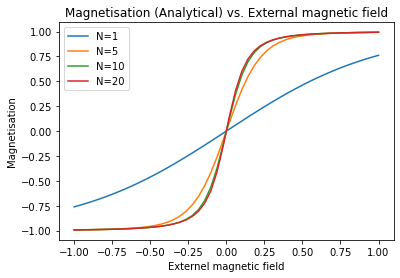
\includegraphics[width=.45\textwidth]{mh-analytic.png}\hfill
    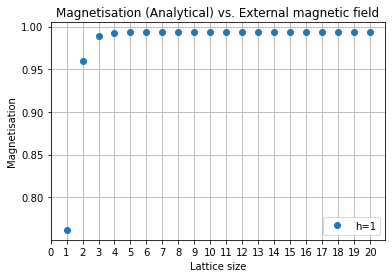
\includegraphics[width=.45\textwidth]{mn-analytic.png}\hfill
    \caption{Magnetisation calculated using analytic expression}
    \label{fig:analytic}
\end{figure}
    In figure \ref{fig:analytic}, we have the plots obtained for magnetisation using an analytic expression. The first subplot shows the magnetisation for different values of the external field. Whereas, the second subplot shows the magnetisation for different lattice sizes with the external magnetic field set at $1$.\\
    We immediately notice that the analytic and numerical solutions agree with each other. We also notice that the analytic solutions converge faster to the large $N$ curve than the numerical solution, in the case of magnetisation vs. external magnetic field. This is not particularly surprising. Again, in the case of magnetisation vs. external magnetic field, the analytic solution converges faster to the expected value of $1$ than the numerical solution.\\
\begin{figure}[h!]
    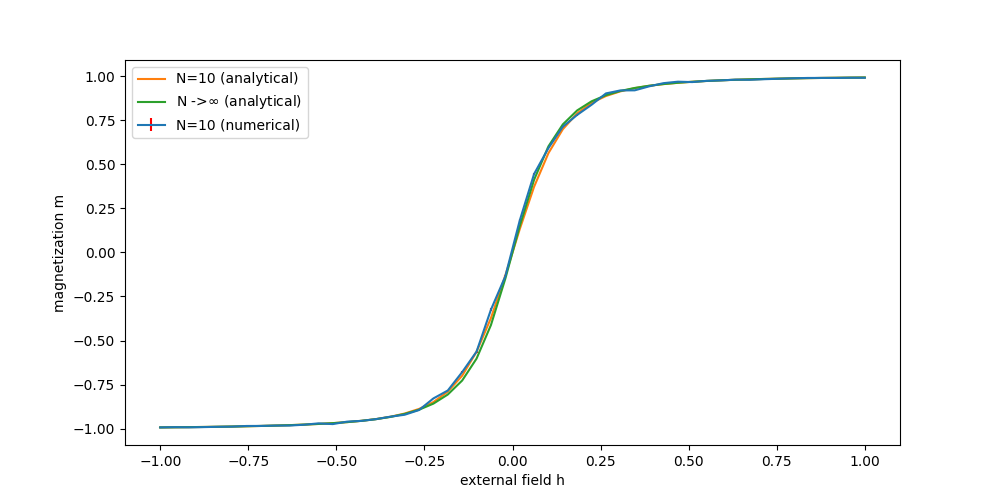
\includegraphics[width=.5\textwidth]{num_vs_anal_N10.png}\hfill
    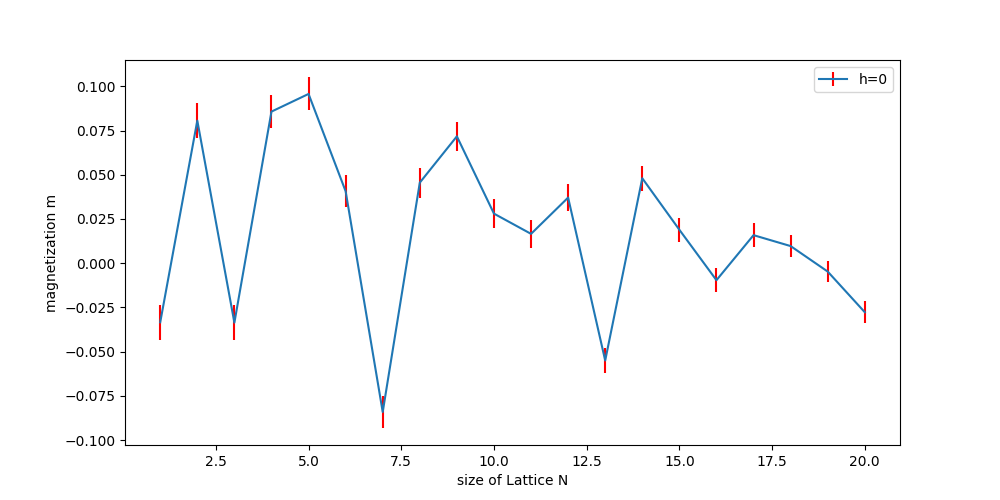
\includegraphics[width=.5\textwidth]{h_0_10000samples.png}\hfill
    \caption{1D Ising model simulation using Metropolis-Hastings algorithm}
    \label{fig:metropolishastings}
\end{figure}
    The errors in the numerical estimations are calculated as simple percentage errors with respect to the analytic calculations. This gives decreasing errors as $N$ grows larger, for both the cases of magnetisation vs. external magnetic field and magnetisation vs. lattice size. The exact values can be found in the output of the $python$ code \verb|Ising1D-BruteForce.py|.\\
    Further, we also implemented the Metropolis-Hastings algorithm for 1D Ising model, and we obtained the figures \ref{fig:metropolishastings}.
    When the external magnetic field h was varied, N was kept constant at 10. You can see that the deviation between the numerical and the analytical solution is very small. Even with the analytical solution with N tending to infinity, the difference is quite small. The curves show a very nearly identical progression. For the variation of N with h fixed at 0, the curve oscillates around the magnetisation m = 0, as expected. With larger N, the fluctuation becomes smaller and approaches 0. What can also be seen very well is that the magnetization shows a very good accuracy even with a small N and is already quite close to 0. The Errors for the Metropolis-Hastings algorithm are defined with standard error by dividing the standard deviation by the sample size's square root.
\end{enumerate}

\end{document}